\documentclass{article}

\usepackage{graphicx}
\usepackage{caption}
\usepackage{subcaption}
\usepackage{booktabs}
\usepackage{csvsimple}
\usepackage{amsmath}
\usepackage{url}

\usepackage[style=authoryear,backend=biber]{biblatex}
% Set library for biblatex
\bibliography{library}

\usepackage{tikz}
\usetikzlibrary{bayesnet}
\usetikzlibrary{positioning}

\title{Predicting positions using Independence Graphs}
\author{Volker Strobel}
\date{\today}

\graphicspath{{img/}}

\begin{document}
\maketitle

% Inducing Features of Random Fields (Pietra)

% I can start with one feature and
% successively include more and more features, until my prediction
% becomes better and better.

% Test on hold-out test see

% Archimedean copulas are an associative class of copulas. Most common
% Archimedean copulas admit an explicit formula, something not
% possible for instance for the Gaussian copula. In practice,
% Archimedean copulas are popular because they allow modeling
% dependence in arbitrarily high dimensions with only one parameter,
% governing the strength of dependence

% Linear regression

% Greedy approach for feature inclusion

% MSE minimizes the expected error
% Another error function minimizes the model

% http://www.r-bloggers.com/modelling-dependence-with-copulas-in-r/

\begin{abstract}
  In this report, we analyze the dependence structure of image
  features and $x,y$-coordinates using linear regression, graphical
  Gaussian models, and vine copulas. The dependencies between color
  and image location are used to build a predictive model for given
  image features. We compare the predictive power of the used models
  using the mean absolute error of the predictions on a hold-out test
  set. The associated uncertainty in the predictions are studied and
  indications are given, how the proposed model can be used in a
  real-world scenario.
\end{abstract}


\section{Introduction \& Problem Statement}

% This could be used in the context of a UAV flight...

% The report will use the notation of \cite{whittaker2009graphical}.


% Idea: use red as an indicator of the environment and add x,y,env as
% prediction goal.

Computer vision tasks---such as object detection, image restoration,
or \emph{localization}--often need a high-dimensional reprentation of
a feature domain. This task can be fulfilled using probabilistic
graphical models and has been used in a variety of applications.

While many problem are studied in the bivariate case only.  However,
combining copula modelling with machine learning techniques was
longtime neglected. Recently, more and more research is focusing on
combining machine learning and regression techniques to tackle
high-dimensional regression problems
\cite{cooke2015vine,elidan2013copulas}.

In this report, we consider the following computer vision localization
problem:

Based on a given patch of an image, we would like to predict, where
the patch was taken in a larger image---the map image. While existing
approaches extract keypoints of the current patch and the map image,
succeeded by finding a homography, these approaches are usually
computationally complex and do not allow for in-depth analyses of the
problem.

This report examines a multivariate problem consisting of five random
variables: average red, green, and blue value of an image patch and
corresponding x, y position of the patch in a larger map image. For
generating the dataset, image patches from a given map image are
generated. These images simulate camera images that could be obtained
during a flight with a micro aerial vehicle (MAV). The problem is
addressed based on two approaches: (i) modifying the environment
(i.e., the map image) to make it better suited for the used approach,
and (ii) modify the approach to make it better suited to the given map
image.

The goal of this report is to select and compare models and use them
for predicting the location ($x,y$-coordinate) of unseen image
patches. To this end, we will infer a dependency model that is able to
capture the multivariate distribution of the sample data. We compare
approaches using linear regression, graphical Gaussian models and vine
copulas.

%Therefore, we address the same problem from three viewing angles.

The remainder of this report is structured as
follows. Section~\ref{sec:methods} introduces the method for
generating the dataset, and for creating the linear least square
predictor, graphical Gaussian models, and vine copulas (we expect the
same results for all models -- see also corollary
Whittaker). Section~\ref{sec:results} shows the obtained results. In
Section~\ref{sec:discussion}, the results are discussed and models are
compared. Finally, in Section~\ref{sec:conclusion}, conclusions and
future research directions are given.


\section{Methods}
\label{sec:methods}

\subsection{Dataset Generation}

Figure~\ref{fig:generation} shows the process of data set
generation. To this end, we will construct a generative model
$p(x,y,R,G,B)$ for the distribution. We decided to create the
generative model, since it allows to construct an image from the
trained model.

In the case of the graphical models, the regression will be performed
by deriving a point estimate from the discrminative model $p(x,y \mid
R,G,B)$ by using one of \emph{mean, median, mode} of the
distribution. Since we will deal with Gaussian distributions, the
three point estimates fall together.

\begin{figure}
  \centering
  \begin{subfigure}[b]{0.4\textwidth}
    \includegraphics[width=\textwidth]{pencils}
    \captionof{figure}{Map image}
    \label{fig:mapimage}
  \end{subfigure}%
~
  \begin{subfigure}[b]{0.4\textwidth}
    \includegraphics[width=\textwidth]{patches}
    \captionof{figure}{Random image patch}
    \label{fig:patch}
  \end{subfigure}
  \caption{Figure~\ref{fig:mapimage} Shows the map image that is used
    for generating the image patches. Figure~\ref{fig:patch} shows one
    sample of the $N = 1000$ image patches that were generated for the
  generation of the data set.}
\label{fig:generation}
\end{figure}

By construction, we know that $x$, $y$ are independent, since the
positions were sampled from independent uniform distributions. This
leads to the data set that can be found in the appendix.

% The presented approach uses simulated data but should be able to
% generalize to real world models.  In a first step, we will select
% suitable features in an iterative approach.

In this setting, the availability of the data is not a problem and new
data can be easily generated. The presented approach is largely
data-driven but also exploits the knowledge of the construction of the
dataset.


For generating the data set, 500 image positions have been sampled
from according to $(x, y) \sim \mathcal{N}(\mu, \Sigma)$, with $\mu =
(320, 240)$ (image center) and $\Sigma = \begin{bmatrix} 107 & 0\\
  0 & 80 \end{bmatrix}$. Therefore, $x$ and $y$ positions are sampled
independently. The standard deviations were chosen, such that 99\,\%
of the data points are expected to be in the ranges $[0, 640]$ and
$[0, 480]$, respectively.


\subsection{First Analysis}

\begin{figure}[h]
  \centering
  \includegraphics[width=0.85\textwidth]{../algo/img/pairs_copuladata.pdf}
  \caption{Analysis of pairs of copula data.}
  \label{fig:pairscopula}
\end{figure}

In our first model, we use three features: the average red, green, and
blue color per image patch. The data set based on $N = 1000$ image
patches can be found in the appendix.

\begin{table}[h]
  \centering
  \begin{tabular}{l|rrrrr}
    red   & 3558  &       &      &       &       \\
    green & 1578  & 3354  &      &       &       \\
    blue  & 1219  & 2749  & 4016 &       &       \\
    x     & -1199 & -427  & -343 & 22900 &       \\
    y     & -871  & -389  & 616  & 467   & 12204 \\
    \midrule
    means & 180   & 154   & 145  & 244   & 192   \\
    \midrule
          & red   & green & blue & x     & y
  \end{tabular}
  \caption{The sample variance matrix of the data set}
\end{table}

\begin{table}[h]
\  \centering
  \begin{tabular}{l|rrrrr}
    red   & 1.00  &       &       &      &      \\
    green & 0.46  & 1.00  &       &      &      \\
    blue  & 0.32  & 0.75  & 1.00  &      &      \\
    x     & -0.13 & -0.05 & -0.04 & 1.00 &      \\
    y     & -0.13 & -0.06 & 0.09  & 0.03 & 1.00 \\
    \midrule
          & red   & green & blue  & x    & y
  \end{tabular}
  \caption{The sample variance matrix of the data set}
\end{table}

\begin{table}                                   
\centering                                      
\begin{tabular}{l|rrrrr}                    
    red   & 1.30  &       &       &       &      \\  
    green & -0.59 & 2.64  &       &       &      \\
    blue  & 0.02  & -1.81 & 2.37  &       &      \\ 
    x     & 0.14  & -0.02 & 0.01  & 1.02  &      \\ 
    y     & 0.13  & 0.24  & -0.32 & -0.01 & 1.06 \\ 
  \midrule
  $R^2$   & 0.23  & 0.62  & 0.58  & 0.02  & 0.06 \\
  \midrule
          & red   & green & blue  & x     & y
\end{tabular}                                   
\caption{Inverse correlation matrix}                        
\label{table:MyTableLabel}                      
\end{table} 

The low values of explained variation for x ($R^2$(x; rest))and y
($R^2$(x; rest)) show that the used approach is not promising. This is
not surprising, given the fact that the colors are non-linearly
distributed in the image (see Figure\ref{fig:colordist} for the
analysis of the colors). Two alternatives could be used to improve the
model's performance. Here, we investigate both.
\begin{itemize}
\item Alternative 1: Change the map image such that higher $R^2$ are
  obtained
\item Alternative 2: Use a more powerful model
\end{itemize}

\subsection{Different map image}

\begin{figure}[h]
  \centering
  %\includegraphics[width=0.7\textwidth]{}
  \caption{A different map image that makes use of the used features.}
  \label{fig:newmap}
\end{figure}

In this case, the image was chosen by manual analysis of the
features. A more interesting case would be to generate the image based
on desired properties of the inverse correlation matrix. 
An ideal inverse correlation matrix would look like:

\begin{table}                                   
\centering                                      
\begin{tabular}{l|rrrrr}                    
    red   & 1.30  &       &       &       &      \\  
    green & -0.59 & 2.64  &       &       &      \\
    blue  & 0.02  & -1.81 & 2.37  &       &      \\ 
    x     & 0.14  & -0.02 & 0.01  & 1.02  &      \\ 
    y     & 0.13  & 0.24  & -0.32 & -0.01 & 1.06 \\ 
  \midrule
  $R^2$   & 0.23  & 0.62  & 0.58  & 0.02  & 0.06 \\
  \midrule
          & red   & green & blue  & x     & y
\end{tabular}                                   
\caption{Inverse correlation matrix}                        
\label{table:MyTableLabel}                      
\end{table} 

%$R^2$   & *  & *  & *  & 1.00  & 1.00 \\

One possible solution would be to set all correlations to a high
value.

\subsection{The backward approach}

\begin{figure}[h]
  \centering
  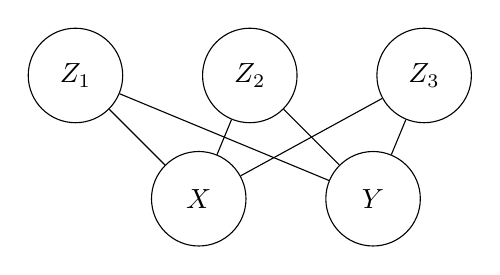
\begin{tikzpicture}[every node={}]
    \node[latent, minimum size=1.2cm] (z1) {$Z_1$} ; %
    \node[latent, right=of z1, minimum size=1.2cm] (z2) {$Z_2$} ; %
    \node[latent, right=of z2, minimum size=1.2cm] (z3) {$Z_3$} ; %
    \node[latent, below right=of z1, minimum size=1.2cm] (x) {$X$} ; %
    \node[latent, below right=of z2, minimum size=1.2cm] (y) {$Y$} ; %
    \edge[-] {z1} {x}; \edge[-] {z1} {y}; \edge[-] {z2} {x}; \edge[-]
    {z2} {y}; \edge[-] {z3} {x}; \edge[-] {z3} {y};
  \end{tikzpicture}
  \caption{The graphical model used for generating ideal images.}
\end{figure}

Knowing the criteria for computing $R^2$, we could construct optimal
images for the given approach. These images will be gradient
images. Since images consist of three channels, we could encode the
information in two channels, and use arbitrary information in the
third channel---and therefore even keep our initial image to a great
extent.


\subsection{Gaussian Graphical Model}

In this subsection, we construct a Gaussian graphical model from our
sample. Two major steps are involved in this procedure: construction
of the independence graph (model selection) and likelihood
inference. To this end, we test for independence using the chi-square
test and fit the variance matrix using iterative proportional
fitting. Since we generated the data, we know that the samples are
identically and independally distributed (i.i.d). The following
conditional independence statements can be read from the graph.

\subsubsection{Model Selection}

While a thresholded exclusions strategy (e.g. corr $<$ 0.1) seems
directly accessible, it does not capture the size and therefore
available information of the sample data.

Therefore, for the model selection, we start with a saturated
graphical model and employ the backward elimination with deviance
difference stopping rule.

This leads to the model in Figure~\ref{fig:}. This leads to a deviance
of $0.13$ on $4$ df with $p$-value of $x$, resulting in the following
$\hat{V}$:

\subsubsection{Inference}

In a first step, the covariance matrix and its inverse are
computed. Then the partial correlations are obtained.

% Construct graph, test for goodness of fit

\subsubsection{Fitting}

Now, we use the IPF algorithm to update the sample variance matrix and
fit it to the given graph.


\subsubsection{Predictions}


From Proposition 6.3.1, we know that the conditional distribution of
$X_b$ given $X_a = a$ is Normal with mean
\begin{align}
  E_{b | a}(X_b) = \mu_b + V_{ba}V^{-1}_{aa}(x_a - \mu_a)
\end{align}
and variance
\begin{align}
  \text{var}_{b|a}(X_b) = V_{bb|a} = V_{bb} - V_{ba}V_{aa}^{-1}V_{ab}
\end{align}
In our case, R,G,B are given, while $x,y$ are
desired. Therefore, we set $X_a = (R, G, B)$ and $X_b = (x,y)$.

\begin{align}
  E_{b | a}(X_b) = \mu_b + V_{ba}V^{-1}_{aa}(x_a - \mu_a)
\end{align}
and variance
\begin{align}
  \text{var}_{b|a}(X_b) = V_{bb|a} = V_{bb} - V_{ba}V_{aa}^{-1}V_{ab}
\end{align}. 


$\mu_b = (320, 240)$ is the center point of the image.

As expected, the conditional mean and the linear least square
predictor are identical (see Corollary 6.3.2). The higher variance in
the x coordinate of the conditional distribution is directly related
to the $R^2$ value.

The GGM is able to infer the independence between the random variables
$R$ and $(x, y)$, leading to more accurate predictions.

\subsection{Vine Copula}

In our final approach, we try to capture the dependence structure
without modifications of the original map image. In order to do so, we
need a more powerful model. The use of \emph{copulas} allows to model
marginal distributions and dependence structure independently,
allowing for convenient and powerful representation of joint
probability distributions. Vine copulas leverage these advantages and
bring the advantages to higher dimensional distributions.

The vine copula approach is based on Sklar's theorem that states that
multivariate distribution can be described by marginal distributions
and the dependence structure----the copulas. Using bivariate copulas
as building blocks, more complex interaction structures can be
achieved by building \emph{vine copulas}--nested sets of connected
trees.

While it is theoretically possible to get $F(x)$ by evaluating it at
\ldots, in practice we have to calculate the inversion of the
(empiricial / pseudo) CDF.
                                          
\section{Results}
\label{sec:results}


\begin{figure}
  \centering
  \begin{subfigure}[b]{0.5\textwidth}
    \includegraphics[width=\textwidth]{dorota_img.pdf}
    \captionof{figure}{Image overlay}
    \label{fig:heatmap}
  \end{subfigure}%
~
  \begin{subfigure}[b]{0.45\textwidth}
    \includegraphics[width=\textwidth]{dorota_contour-crop}
    \captionof{figure}{Contour plot}
    \label{fig:contour}
  \end{subfigure}
  \caption{Example of the visualization of the predictions using RGB =
    (100, 70, 200)}
\label{fig:predvisualization}
\end{figure}


\begin{figure}
  \centering
  \begin{subfigure}[b]{0.5\textwidth}
    \includegraphics[width=\textwidth]{tree1}
    \captionof{figure}{Image overlay}
    \label{fig:heatmap}
  \end{subfigure}%
~
  \begin{subfigure}[b]{0.45\textwidth}
    \includegraphics[width=\textwidth]{contour_copula}
    \captionof{figure}{Contour plot}
    \label{fig:contour}
  \end{subfigure}
  \caption{Example of the visualization of the predictions using RGB =
    (100, 70, 200)}
\label{fig:predvisualization}
\end{figure}

A visualization of the used bivariate copulas can be found in the
appendix (\ref{sec:copulas}).
     
\section{Discussion}
\label{sec:discussion}

This report presented three different approaches for modeling the
dependencies in a five-dimensional regression problem. The presented
results indicate the suitability of our approach. While the initially
chosen image did not allow for modeling the dependency using a
parametric model, the modification of the map image allowed to
continue with the analysis.

In a real-world setting, run-time and computational complexity will be
crucial which we left out here.

An interesting future research direction will be the inclusion of time
dependence: in a real-world scenario, images will not be i.i.d but
highly correlated.


\section{Conclusion}
\label{sec:conclusion}

%In this report, the suitability of independence graphs for computer
%vision-based localization was shown. While the straight-forward
%application of linear regression was not able to capture the structure
%in the generated dataset, a modification of the image underlying the
%data set allowed to generate a simple and effective model, which lead
%to low mean squared errors.

In this report, we compared linear regression, graphical Gaussian
models and vine copulas for the dependence modeling of variables in a
computer vision task. 

\printbibliography
\appendix

\section{Supplementary Material}

\section{Visualization of the used copulas}
\label{sec:copulas}

\subsection{Tree 1}

\subsection{Tree 2}

\subsection{Tree 3}


\section{Dataset with average red, green, and blue values}
\begin{center}
  \csvautotabular{all_vals.csv}
\end{center}


\section{Technical Report}
\label{sec:technical}

The code for generating the graphs and yielding the results presented
in this report was written in \texttt{R}. The used data is saved in
CSV format. Both can be found on GitHub:\\
\noindent\url{https://github.com/Pold87/decision-theory}\\

The section on Graphical Gaussian Models made use of the packages
\texttt{gRim, gRbase} and \texttt{Rgraphviz} for the visualization.\\

The section on VineCopula used the packages \texttt{copula} and
\texttt{VineCopula}.

\end{document}
